%%%%%%%%%%%%%%%%%%%%%%%%%%%%%%%%%%%%%%%%%
% Simple Sectioned Essay Template
% LaTeX Template
%
% This template has been downloaded from:
% http://www.latextemplates.com
%
% Note:
% The \lipsum[#] commands throughout this template generate dummy text
% to fill the template out. These commands should all be removed when 
% writing essay content.
%
%%%%%%%%%%%%%%%%%%%%%%%%%%%%%%%%%%%%%%%%%

%----------------------------------------------------------------------------------------
%	PACKAGES AND OTHER DOCUMENT CONFIGURATIONS
%----------------------------------------------------------------------------------------

\documentclass[12pt]{article} % Default font size is 12pt, it can be changed here

\newcommand{\normalsubparagraph}[1]{\subparagraph{\textnormal{#1}}}

\usepackage{geometry} % Required to change the page size to A4
\geometry{a4paper} % Set the page size to be A4 as opposed to the default US Letter

\usepackage{graphicx} % Required for including pictures
\usepackage{enumitem}
\usepackage{float} % Allows putting an [H] in \begin{figure} to specify the exact location of the figure
\usepackage{wrapfig} % Allows in-line images such as the example fish picture

\usepackage{lipsum} % Used for inserting dummy 'Lorem ipsum' text into the template

\linespread{1.2} % Line spacing

%\setlength\parindent{0pt} % Uncomment to remove all indentation from paragraphs

\graphicspath{{./Pictures/}} % Specifies the directory where pictures are stored

%para escribir en español
\usepackage[utf8x]{inputenc}
\usepackage[spanish]{babel}
\usepackage{subcaption}

\newcommand{\normalparagraph}[1]{\paragraph{\textnormal{#1}}}

\begin{document}

%----------------------------------------------------------------------------------------
%	TITLE PAGE
%----------------------------------------------------------------------------------------

\begin{titlepage}

\newcommand{\HRule}{\rule{\linewidth}{0.5mm}} % Defines a new command for the horizontal lines, change thickness here

\center % Center everything on the page

\textsc{\LARGE Taller de Iniciación a los Sistemas Ciber-Físicos}\\[1.5cm] % Name of your university/college
\textsc{\Large Curso 2024}\\[0.5cm] % Major heading such as course name
%\textsc{\large Grupo XX}\\[0.5cm] % Minor heading such as course title

\HRule \\[0.4cm]
{ \huge \bfseries CyberRoomCount}\\[0.4cm] % Title of your document
\HRule \\[1.5cm]

\begin{minipage}{0.4\textwidth}
\begin{flushleft} \large
\emph{Autores:}\\
Diego Forlong \textsc{}\\ % Your name
Lucía Gavilanes  \textsc{}\\ % Your name
Santiago Mendoza \textsc{}\\ % Your name
Cynthia Velazquez \textsc{}\\ % Your name
\end{flushleft}
\end{minipage}
~
\begin{minipage}{0.4\textwidth}
\begin{flushright} \large
\emph{Supervisores:} \\
Eduardo Grampin \textsc{}% Supervisor's Name
\\
Joaquín Veirana \textsc{}
\end{flushright}
\end{minipage}\\[4cm]

{\large \today}\\[3cm] % Date, change the \today to a set date if you want to be precise

%\includegraphics{Logo}\\[1cm] % Include a department/university logo - this will require the graphicx package

\vfill % Fill the rest of the page with whitespace

\end{titlepage}

%----------------------------------------------------------------------------------------
%	TABLE OF CONTENTS
%----------------------------------------------------------------------------------------

\tableofcontents % Include a table of contents

\newpage % Begins the essay on a new page instead of on the same page as the table of contents 

%----------------------------------------------------------------------------------------
%	INTRODUCTION
%----------------------------------------------------------------------------------------

\section{Introducción} % Major section


%------------------------------------------------

\subsection{Objetivos del proyecto} % Sub-section
\normalparagraph{El propósito del proyecto es observar, estudiar y analizar el flujo de entrada y salida de estudiantes, considerando el impacto de la cantidad de personas en el aula. Activando actuadores bajo ciertas condiciones, a modo de recaudador de datos para analizar posteriormente. }


%------------------------------------------------

\subsection{Materiales} % Sub-section
\begin{enumerate}[itemsep=1pt] 
    \item Sensor de temperatura y humedad: dht11
    \item Sensor de distancia: hc-sr04 (2)
    \item Placa: ESP8266
\end{enumerate}

%------------------------------------------------

%----------------------------------------------------------------------------------------
%	MAJOR SECTION 1
%----------------------------------------------------------------------------------------

\section{Presentación del proyecto} % Major section


%------------------------------------------------

\subsection{Etapa inicial - Planificación} % Sub-section
\normalparagraph {Se planea hacer el proyecto con una maqueta que simule un salón, ya que hacerlo a escala real consumiría muchos recursos y dificultaría la etapa de pruebas.}

\subsubsection{Maqueta} % Sub-sub-section



\begin{figure}[h!]
\centering
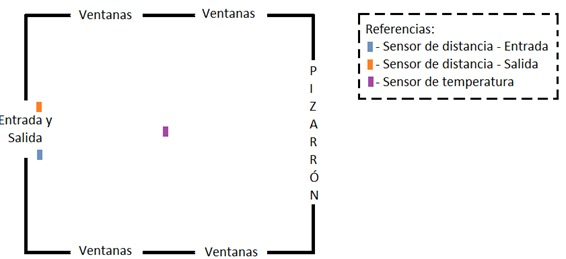
\includegraphics[width=0.79\linewidth]{Pictures/salon.jpeg}
\setcounter{subfigure}{2}%
\caption{Esquema salón}\label{fig:esquema}
\end{figure}

\normalparagraph {Este proceso llevó aproximadamente dos semanas en total. Aun así, no fue continuo, ya que se esperó hasta saber qué sensores se utilizarían y sus dimensiones antes de proceder a fijar las piezas.}

\begin{center}
\begin{minipage}[b]{0.45\textwidth}
  \centering
  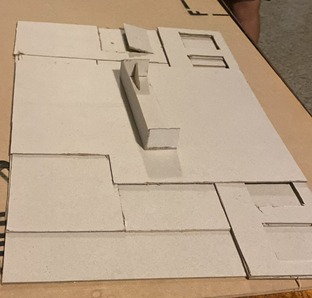
\includegraphics[width=\linewidth]{Pictures/recortes_maqueta.jpeg}
  \captionof{figure}{Comienzando}\label{fig:recortes}
\end{minipage}
\hspace{0.5cm} % Espacio horizontal entre las minipages
\begin{minipage}[b]{0.45\textwidth}
  \centering
  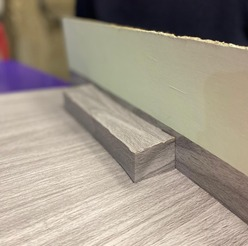
\includegraphics[width=\linewidth]{Pictures/proceso_maqueta_1.jpeg}
  \captionof{figure}{Iniciando el ensamblaje}\label{fig:proceso1}
\end{minipage}

\vspace{0.5cm} % Espacio vertical entre las dos filas de minipages

\begin{minipage}[b]{0.45\textwidth}
  \centering
  \includegraphics[width=\linewidth]{Pictures/proceso_maqueta_2.jpeg}
  \captionof{figure}{Terminando el ensamblaje}\label{fig:proceso2}
\end{minipage}
\hspace{0.5cm} % Espacio horizontal entre las minipages
\begin{minipage}[b]{0.45\textwidth}
  \centering
  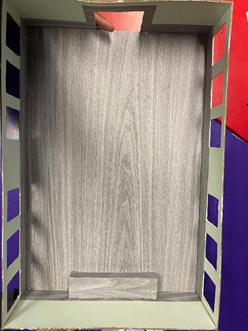
\includegraphics[width=\linewidth]{Pictures/proceso_maqueta_3.jpeg}
  \captionof{figure}{Finalizada}\label{fig:proceso3}
\end{minipage}
\end{center}



%\begin{center}
%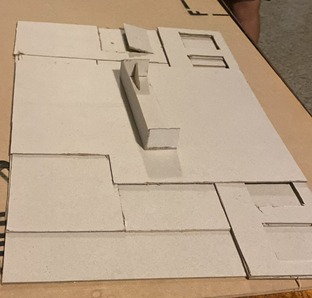
\includegraphics[width=0.40\textwidth]{Pictures/recortes_maqueta.jpeg}

%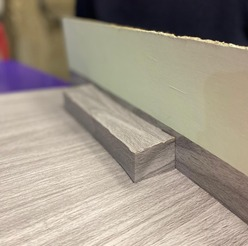
\includegraphics[width=0.30\textwidth]{Pictures/proceso_maqueta_1.jpeg}

%\includegraphics[width=0.40\textwidth]{Pictures/proceso_maqueta_2.jpeg}

%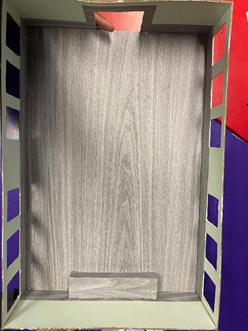
\includegraphics[width=0.40\textwidth]{Pictures/proceso_maqueta_3.jpeg}

%\end{center}

\normalparagraph {Un problema que se presentó al pegar las piezas de la maqueta: Tras su fijación, las paredes comenzaron a deformarse por a la ausencia de contención en la parte superior. Para solucionarlo, se diseñaron esquineros con el fin de mantener las paredes en su forma original.}


\begin{center}
\begin{minipage}[b]{0.4\textwidth}
  \centering
  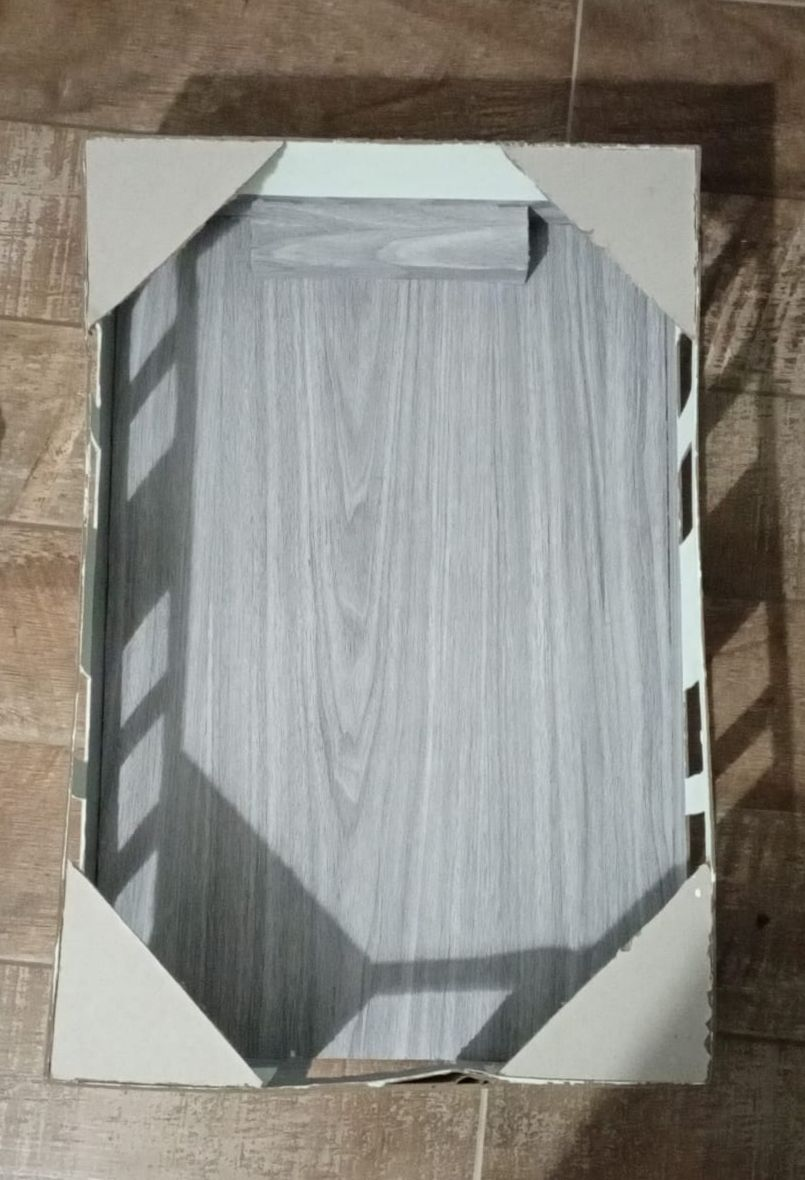
\includegraphics[width=\linewidth]{Pictures/Maqueta con soportes.jpg}
  \captionof{figure}{Maqueta con soportes}\label{fig:maqueta}
\end{minipage}
\end{center}

%------------------------------------------------

\subsection{Etapa intermedia - Uso de sensores} % Sub-section
\normalparagraph {Se comenzarán utilizando tres sensores que son los elementales para poder cumplir con el objetivo del proyecto. }


\begin{center}
\begin{minipage}[c]{0.75\textwidth} % Ajusta la anchura de la minipage
  \centering
  \includegraphics[width=\linewidth]{Pictures/Diseño de prototipo.jpg}
  \captionof{figure}{Prototipo de conexión inicial}\label{fig:prototipo}
\end{minipage}
\end{center}




\normalparagraph {Pruebas de conexión con sensores:}
\normalsubparagraph {Sensor de distancia - Conexiones (sensor-placa):}

\begin{enumerate}[itemsep=1pt] % Ajusta el espacio entre items
    \item GND - GND
    \item Echo - D5
    \item Trig - D6
    \item Vcc – VU o 3.3V
\end{enumerate}

%\begin{enumerate}
 %   \item GND - GND
  %  \item Echo - D5
   % \item Trig - D6
    %\item Vcc – VU o 3.3V
%\end{enumerate}

\begin{center}
\begin{minipage}[c]{0.4\textwidth} % Ajusta la anchura de la minipage
  \centering
  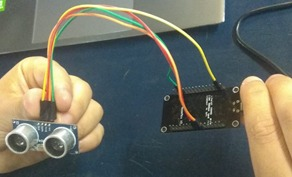
\includegraphics[width=\linewidth]{Pictures/Sensor distancia.jpg}
  \captionof{figure}{Sensor de distancia}\label{fig:sensor-distancia}
\end{minipage}
\end{center}

%\begin{center}
%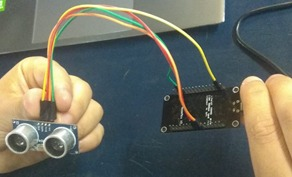
\includegraphics[width=0.50\textwidth]{Pictures/Sensor distancia.jpg}
%\end{center}

\normalsubparagraph {Sensor de temperatura - Conexiones (sensor-placa):}
\begin{enumerate}[itemsep=1pt]
    \item GND - GND
    \item OUTPUT - D7
    \item Vcc – 3.3V
\end{enumerate}

\begin{center}
\begin{minipage}[c]{0.3\textwidth} % Ajusta la anchura de la minipage
  \centering
  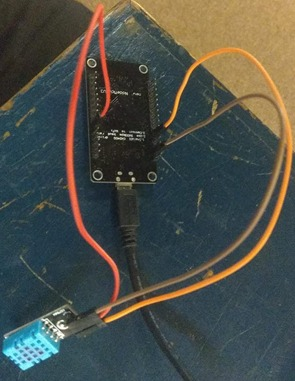
\includegraphics[width=\linewidth]{Pictures/Sensor temperatura.jpg}
  \captionof{figure}{Sensor de \mbox{temperatura}}\label{fig:sensor-temperatura}
\end{minipage}
\end{center}

%\begin{center}
%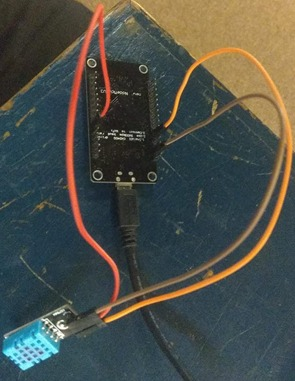
\includegraphics[width=0.40\textwidth]{Pictures/Sensor temperatura.jpg}
%\end{center}

\normalsubparagraph{Sensores conectados al mismo tiempo:}

\begin{center}
\begin{minipage}[c]{0.65\textwidth} % Ajusta la anchura de la minipage
  \centering
  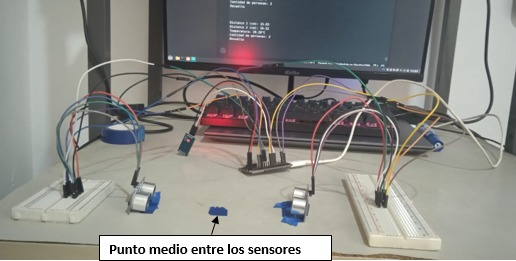
\includegraphics[width=\linewidth]{Pictures/Todos los sensores conectados.jpg}
  \captionof{figure}{Todos los sensores conectados}\label{fig:todos-sensores}
\end{minipage}
\end{center}

%\begin{center}
%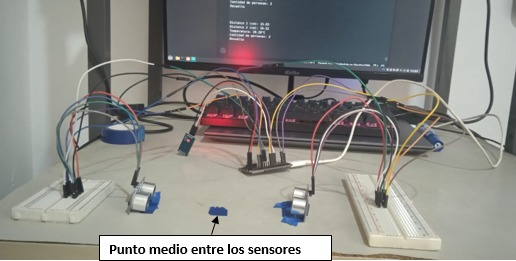
\includegraphics[width=0.65\textwidth]{Pictures/Todos los sensores conectados.jpg}
%\end{center}


\normalsubparagraph{Como se puede notar en la imagen, se conectaron los sensores de distancia y el de temperatura y humedad al mismo tiempo en la placa. Se utilizaron protoboards para poder aumentar la distancia entre los señores y la placa, se plantea la idea de usar cables más largos y no incluirlas en la parte final. }
%------------------------------------------------

%------------------------------------------------

%------------------------------------------------

%------------------------------------------------

%------------------------------------------------

\subsubsection{Limitaciones del prototipo y sensores} % Sub-sub-section
\normalparagraph{Se realizan pruebas para poder conocer las restricciones que hay al usar una maqueta, tomando en cuenta ciertas precondiciones para el funcionamiento esperado, y los sensores presentados anteriormente. Se han contemplado escenarios en los cuales el sistema podría experimentar fallos, resultando en salidas inesperadas:}
\normalparagraph{Limitaciones por sensores:}

\begin{enumerate}
    \item Prueba: Pasar un objeto a 1,0 cm del sensor.  
Resultado esperado: La distancia mostrada en la pantalla debe ser 1,0 cm.
Resultado obtenido: La distancia que se imprime en la pantalla es 14,0 cm.
    \item Prueba: Se pasa un objeto a una velocidad mayor que la que pueden captar los sensores.
Resultado esperado: No toma nada.
Resultado obtenido: Hace sumas o restas erróneas
\end{enumerate}
\newpage
\subparagraph{Observación: Esta también se podría considerar como una limitación de código, ya que, si bien los sensores necesitan poder captar al objeto por cierto tiempo, en el código este se aumentó, con el objetivo de evitar salidas inesperadas. Este tipo de error se pudo solucionar realizándole cambios al código inicial.}

\normalparagraph{Limitaciones por condiciones:}
\begin{enumerate}
    \item Prueba: Se hace pasar un objeto exactamente por el punto medio entre ambos sensores.
Resultado esperado: El contador debería ajustarse sumando o restando uno, dependiendo del lado por el que el objeto pase.
Resultado obtenido: El contador no se modifica, se mantiene igual.
\end{enumerate}

\normalsubparagraph{Esto sucede porque en las precondiciones las personas entran por un lado y salen por el otro, lo cual provocaría que el punto medio sea una parte de la entrada en la que no se puede contar.}
%------------------------------------------------
%------------------------------------------------

\subsubsection{Plataforma ThingSpeak:} % Sub-sub-section
\normalparagraph{Se hicieron algunas pruebas con los sensores y la plataforma de ThingSpeak para poder entender cómo funcionaba. Siendo esta la primera gráfica obtenida (aún no se esperaban obtener datos concretos):}

\normalparagraph{Grafica que representa la temperatura:}

\begin{center}
\begin{minipage}[c]{0.65\textwidth} % Ajusta la anchura de la minipage
  \centering
  \includegraphics[width=\linewidth]{Pictures/Primera gráfica.jpg}
  \captionof{figure}{Primera gráfica}\label{fig:primera-grafica}
\end{minipage}
\end{center}

%\begin{center}
%\includegraphics[width=0.55\textwidth]{Pictures/Primera gráfica.jpg}
%\end{center}
%------------------------------------------------

\subsubsection{ Recolección de datos} % Sub-sub-section
\normalparagraph{Para la recolección de datos se tuvieron que implementar cambios en la idea inicial, ya que la propuesta había sido pensada para un espacio lo suficientemente grande como para marcar una parte de entrada y otra de salida. Sin embargo, al momento de extraer datos, se decidió colocarlo en un pasillo, el cual, al ser más estrecho, presentó una dificultad al momento de usar los sensores de la manera anteriormente planteada. Por lo tanto, se decidieron alinear como se muestra en la siguiente imagen:}


\begin{center}
\begin{minipage}[c]{0.45\textwidth} % Ajusta la anchura de la minipage
  \centering
  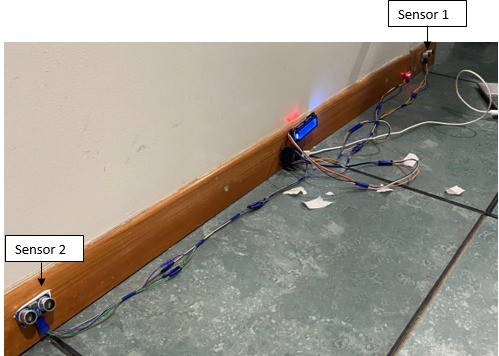
\includegraphics[width=\linewidth]{Pictures/Sensores distancia - Colocados.jpg}
  \captionof{figure}{Sensores de distancia \mbox{colocados}}\label{fig:sensores-distancia}
\end{minipage}
\end{center}

%\begin{center}
%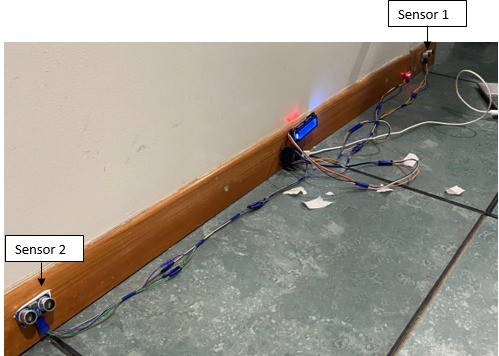
\includegraphics[width=0.50\textwidth]{Pictures/Sensores distancia - Colocados.jpg}
%\end{center}

\normalparagraph{La lógica de funcionamiento para esta distribución es que, si la persona es captada primero por el sensor 1 y luego por el sensor 2, entonces se suma, en caso de que el orden sea invertido, se resta.
Para extraer los datos con el sensor de temperatura no se realizaron cambios en la idea inicial:}

\begin{center}
\begin{minipage}[c]{0.45\textwidth} % Ajusta la anchura de la minipage
  \centering
  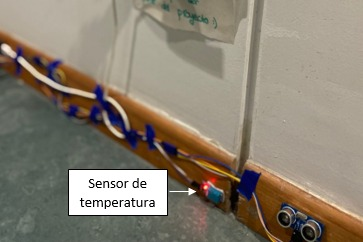
\includegraphics[width=\linewidth]{Pictures/Sensor temperatura - Colocado.jpg}
  \captionof{figure}{Sensor de temperatura \mbox{colocado}}\label{fig:sensor-temperatura}
\end{minipage}
\end{center}

%\begin{center}
%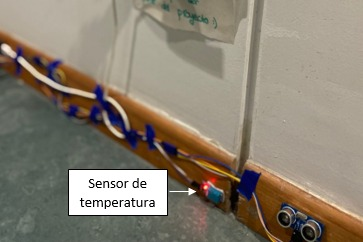
\includegraphics[width=0.65\textwidth]{Pictures/Sensor temperatura - Colocado.jpg}
%\end{center}

%------------------------------------------------

\subsection{Etapa final - Análisis} % Sub-section
\normalparagraph{Se realizó un proceso de filtrado de los datos en el cual eliminamos datos repetidos que no aportaran información valiosa, por ejemplo, la recolección de datos de un domingo en el cual el movimiento es prácticamente nulo en el pasillo.}

\normalparagraph{En la tabla se pueden observar las diferencias de horario (así como de fecha) de la toma de datos, pudiéndose ver las variaciones de personas a lo largo del día.}

\normalparagraph{Respecto a los datos esperados, por las complicaciones al momento de materializar la idea del proyecto, fueron en algunos aspectos distintos a los esperados, por ejemplo, al ser los datos tomados en un pasillo y no un salón cerrado, no es acorde el cambio de temperatura con la cantidad de gente que cuenta el sensor (que, de hecho, ni siquiera es “cantidad de gente en el salón”, sino más bien “cantidad de gente que va hacia un lado o el otro”). Aun así, es importante destacar que el actuador si respondió a los cambios de temperatura que debía, habiéndose inicializado cuando la temperatura bajó de 19°, y apagándose cuando superó la misma. }

\normalparagraph{Datos del sensor de distancia:}

\begin{center}
\begin{minipage}[c]{0.75\textwidth} % Ajusta la anchura de la minipage
  \centering
  \includegraphics[width=\linewidth]{Pictures/Gráfica cantidad de personas.jpg}
  \captionof{figure}{Gráfica de cantidad de personas}\label{fig:grafica-personas}
\end{minipage}
\end{center}

%\begin{center}
%\includegraphics[width=0.65\textwidth]{Pictures/Gráfica cantidad de personas.jpg}
%\end{center}

\normalparagraph{Se puede observar que los datos son concordantes con los horarios, por ejemplo, del domingo y el miércoles (que fue feriado), no hay datos recolectados. En el resto de los días, empieza a crecer la cantidad de gente que “entra” a la hora de la mañana (concuerda con el horario de trabajo), y a disminuir acercada la tarde/noche, cuando la gente “sale” (fin de la jornada).
Se podrían transpolar estos datos a “inicio” de una clase y “final” de la misma, respectivamente.}

\normalparagraph{Datos del sensor de temperatura y el actuador:}


\begin{center}
\begin{minipage}[c]{0.65\textwidth} % Ajusta la anchura de la minipage
  \centering
  \includegraphics[width=\linewidth]{Pictures/Gráfica temperatura.jpg}
  \captionof{figure}{Gráfica de temperatura}\label{fig:grafica-temperatura}
\end{minipage}
\end{center}


%\begin{center}
%\includegraphics[width=0.65\textwidth]{Pictures/Gráfica temperatura.jpg}
%\end{center}

\normalparagraph{Como se explicó anteriormente, no se puede establecer una relación entre la temperatura y la cantidad de gente que simplemente pasaba, pero si se puede observar que cuando hay menos de 19°, el actuador se prende.}

\begin{center}
\begin{minipage}[c]{0.60\textwidth} % Ajusta la anchura de la minipage
  \centering
  \includegraphics[width=\linewidth]{Pictures/Gráfica actuador.jpg}
  \captionof{figure}{Gráfica del actuador}\label{fig:grafica-actuador}
\end{minipage}
\end{center}

%\begin{center}
%\includegraphics[width=0.55\textwidth]{Pictures/Gráfica actuador.jpg}
%\end{center}

\paragraph{Aclaración: Pese a que puede parecer que la gráfica esá compuesta por líneas rectas, en realidad está formada de varios puntos. Por este motivo, en algunos sectores puede parecer que está tomando los valores 0 y 1 al mismo tiempo, pero este no es el caso. Esto se debe a que el cambio de un decimal entre un momento y otro pueda ocasionar el encendido o apagado del actuador.}

\normalparagraph{En cuanto a la gráfica del actuador, indica si el sistema considera necesario activar el aire acondicionado para ajustar la temperatura ambiente. Los valores en la gráfica oscilan entre 0 y 1:}
\normalsubparagraph{  •	0: No se requiere la intervención del actuador. Esto ocurre cuando la temperatura está dentro del rango considerado confortable o normal}
\normalsubparagraph{ • 1: Se necesita la intervención del actuador. Esto sucede cuando la temperatura es demasiado baja o demasiado alta, y se requiere que el aire acondicionado ajuste la temperatura para alcanzar niveles confortables.}

\normalparagraph{La gráfica, por tanto, muestra cuándo el sistema detecta temperaturas no deseables y activa el aire acondicionado en respuesta, asegurando un ambiente confortable.}

\normalparagraph{Por las dificultades de corresponder la temperatura con la cantidad de gente en el salón, optamos por poner la temperatura borde en 19° (temperatura promedio en el pasillo en esta época del año), para poder de esta manera mostrar cuando el actuador se iniciase.}


%----------------------------------------------------------------------------------------
%	CONCLUSION
%----------------------------------------------------------------------------------------
\newpage
\section{Conclusión} % Major section

\normalparagraph{Conclusiones del uso de sensores:}
\normalsubparagraph {Durante el desarrollo del proyecto, se pudo constatar la viabilidad del uso de sensores para la extracción de datos. Sin embargo, se identificó que en ciertas instancias los datos obtenidos no fueron tan precisos como se esperaba. Esta limitación podría haberse solucionado mediante el uso de un mayor número de sensores o adquiriendo dispositivos de mayor calidad.
}
\normalparagraph{Conclusiones sobre la aplicabilidad del proyecto:}
\normalsubparagraph {Conforme a los objetivos establecidos, el proyecto se enfocó en la implementación de un sistema capaz de recopilar y analizar datos mediante la integración de sensores con la plataforma ThingSpeak. Este enfoque facilitó la extracción y filtrado de datos, permitiendo la generación de gráficos para el análisis del entorno del salón de manera efectiva. 
La información obtenida podría ser utilizada para determinar las horas y clases con mayor y menor afluencia de estudiantes, proporcionando a los profesores información útil para la selección de salones más adecuados para sus clases. Además, poder medir la temperatura en tiempo real, permitiría la automatización de actuadores en función de las condiciones ambientales.}
%----------------------------------------------------------------------------------------
%	BIBLIOGRAPHY
%----------------------------------------------------------------------------------------


\begin{thebibliography}{99} % Bibliography - this is intentionally simple in this template

\bibitem[HC-SR04 Ultrasonic Sensor]{CodigoSensorDistancia}
Código de sensor de distancia. Disponible en: 
\begin{minipage}[t]{0.8\textwidth}
\url{https://techatronic.com/hc-sr04-ultrasonic-sensor-working-with-esp8266-nodemcu/}
\end{minipage}

\bibitem[ESP8266 DHT11 Sensor]{CodigoSensorTemperatura}
Código de sensor de temperatura. Disponible en: 
\begin{minipage}[t]{0.8\textwidth}
\url{https://newbiely.com/tutorials/esp8266/esp8266-dht11}
\end{minipage}

\bibitem[Display RG1602A]{CodigoDisplay}
Código de display. Disponible en: 
\begin{minipage}[t]{0.8\textwidth}
\url{https://randomnerdtutorials.com/esp32-esp8266-i2c-lcd-arduino-ide/}
\end{minipage}


\end{thebibliography}
%----------------------------------------------------------------------------------------

\end{document}